\chapter{Implementation}\label{chapter:core_implementation}

\section{Stereo Camera}

Like Structure from Motion, the stereo depth instance is a ROS node which is given images and image poses from the xVIO state estimator. As the state estimator was in its final development stages during my thesis, camera images and a ground truth camera pose from the simulation were used instead as input for the stereo algorithm. Note that only one camera pose is given as the second one is derived in a straight forward manner, given the fixed hardware baseline.

\subsection{Input Handling}
The input of the images as well as the base link pose are received using ROS subscribers. Despite publishing these simulated Gazebo topics at equal rates however, they did not arrive simultaneously. Note that this would be resolved when working with the actual xVIO state estimator as it uses the tracking camera's image and supplies further nodes with that same image as well as the pose with synchronized timestamps.

The pose is only required for the transfer of the created points from the camera frame to the world frame. Therefore, the two input images were processed into a depth image in a single step and only after were all three inputs used in order to create the point cloud. 

The node handled this shortcoming of asynchronous sensor messages by manually picking the pose which temporally closest corresponds to the image's timestamp. This was possible as the image processing step dominates the computation time of the input handling and the pose can thus be continuously updated in the meantime to best fit the images.


\subsection{Disparity Creation}

\subsection{Point Cloud Creation}
The final output of the node is a generated point cloud in the world frame together with two poses representing the camera locations of the generated point cloud.

\subsection{Transform Overview}

A critical part of navigation is always the consistency of the coordinate systems in which quantities are represented. Hereafter is a display of the present coordinate systems in the stereo camera setup.

\subsection{Switching}

In order to achieve the final desired perception mechanism of flying laterally with SFM and using a stereo camera depth node at low altitudes, one needs to switch between the two alternatives.

The obvious decision to use in the switching mechanism is the drone's current altitude above ground. This could be achieved by analyzing the generated point cloud at a given iteration to determine the median altitude which indicates the altitude above ground. This however is avoidable computational overhead.

As mentioned in \cref{sec:state_estimator} the drone has a laser range finder on board. This allows us to get an estimate of the altitude above ground at any given moment without the need for image processing.

Therefore, the switching is performed by using a separate ROS subscriber which continuously checks the LRF's measurement and activates or deactivates the SFM node and stereo node respectively.

\clearpage %HERE
\begin{figure}
    \centering
    \includegraphics[scale=0.17]{images/preparation/stereo/switching.png}
    \caption{Laser Ranger Finder Based Switch between Depth Sources}
\end{figure}

\subsection{Landing Site Detection without Lateral Motion}

Taking off vertically with the drone in the simulation, the first landing site without lateral motion was found.

\begin{figure}
    \centering
    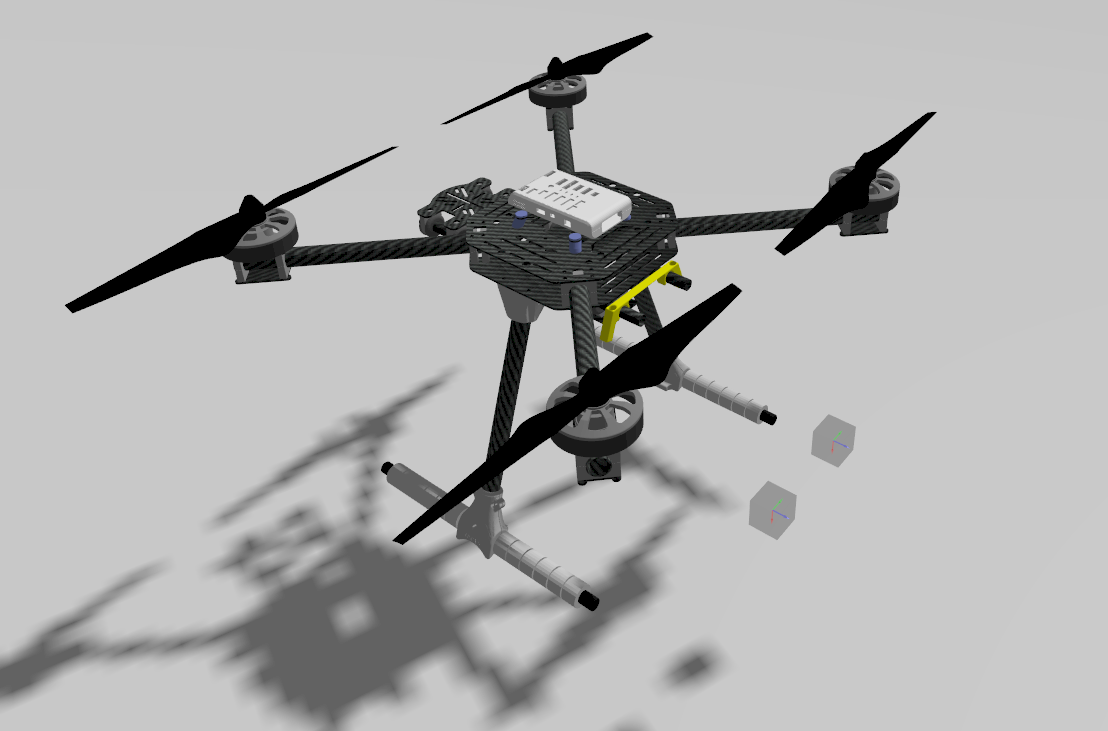
\includegraphics[scale=0.32]{images/preparation/stereo/drone_with_stereo_cam.png}
    \caption{Stereo camera on drone indicated by opaque boxes}
\end{figure}

\begin{figure}
    \centering
    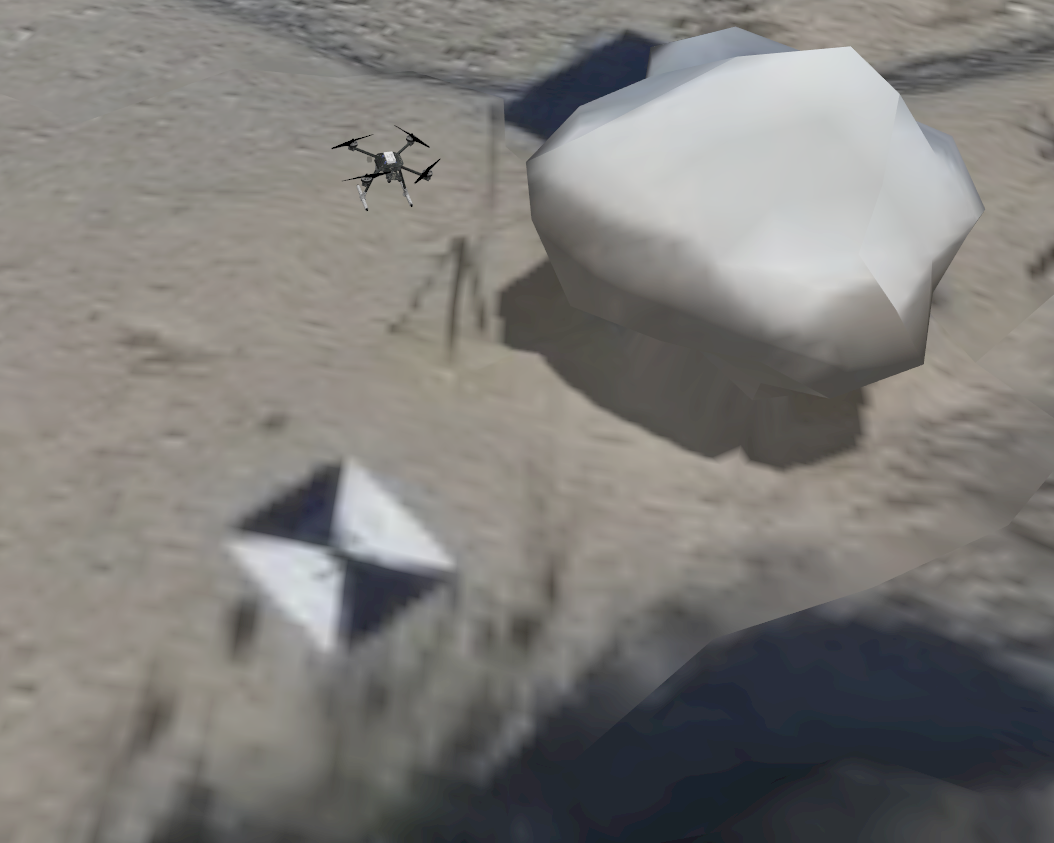
\includegraphics[scale=0.34]{images/preparation/stereo/ascent_sim.png}
    \caption{Drone during vertical ascent in simulation}
\end{figure}

\begin{figure}
    \centering
    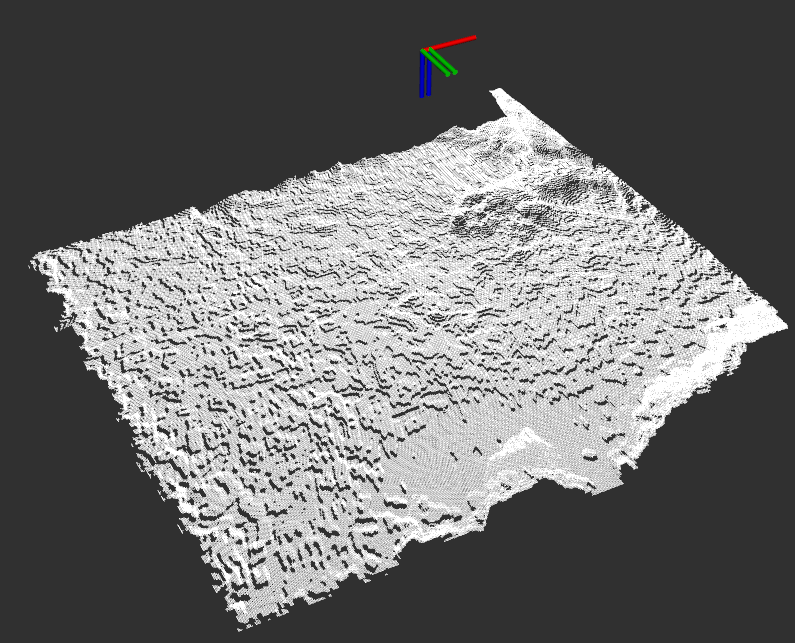
\includegraphics[scale=0.45]{images/preparation/stereo/stereo_pointcloud.png}
    \caption{RViz visualization of created point cloud from stereo camera}
\end{figure}
\clearpage %HERE

\begin{figure}
    \centering
    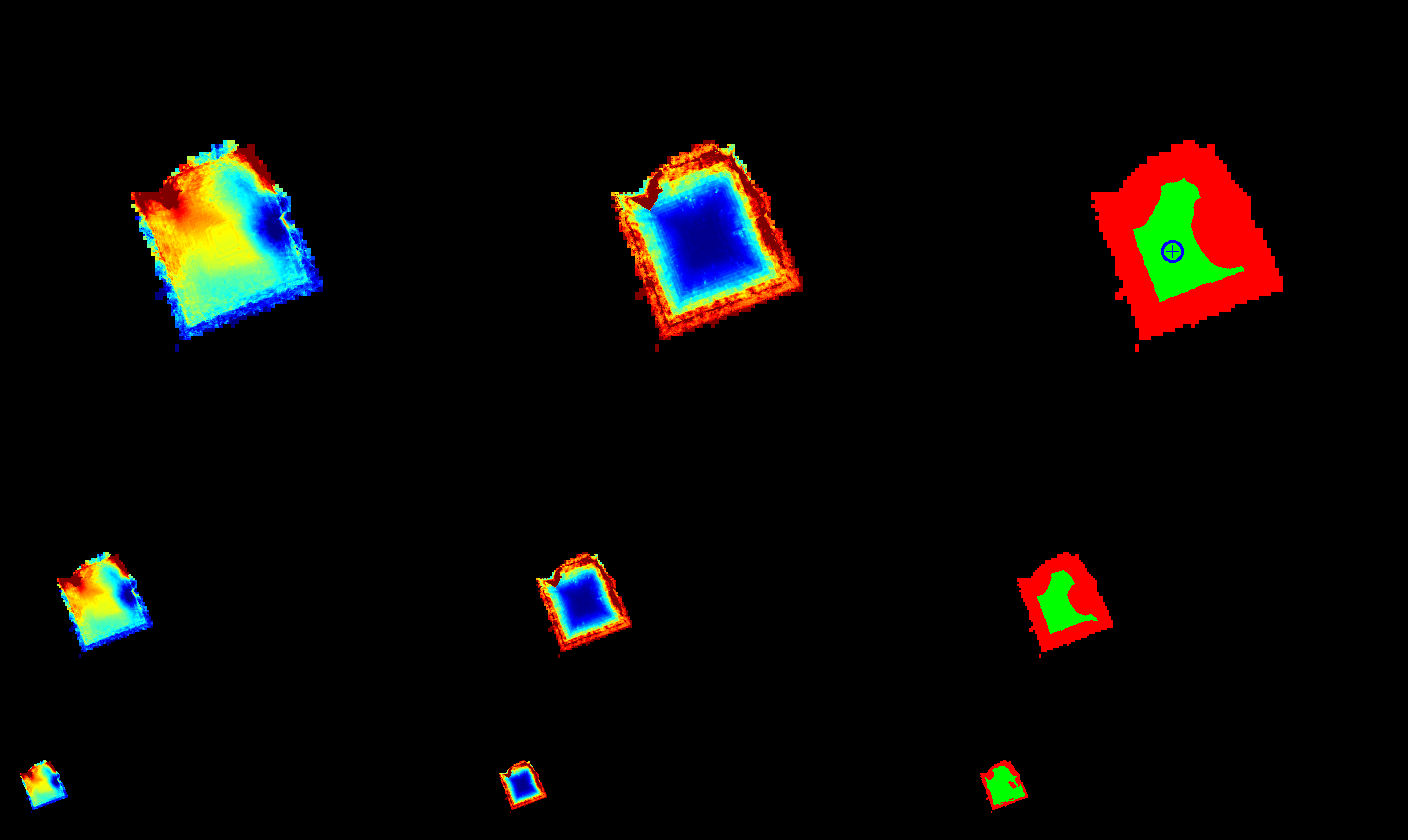
\includegraphics[scale=0.25]{images/preparation/stereo/lsd_ascent.png}
    \caption{LSD Debug output displaying LORNA's first detected landing site during vertical motion}
\end{figure}

\subsection{Qualitative Practical Analysis}

Once implemented the landing site detection instance could be supplied by the stereo depth node. The result thereof can be seen below:

\begin{figure}[ht!]
    \centering
    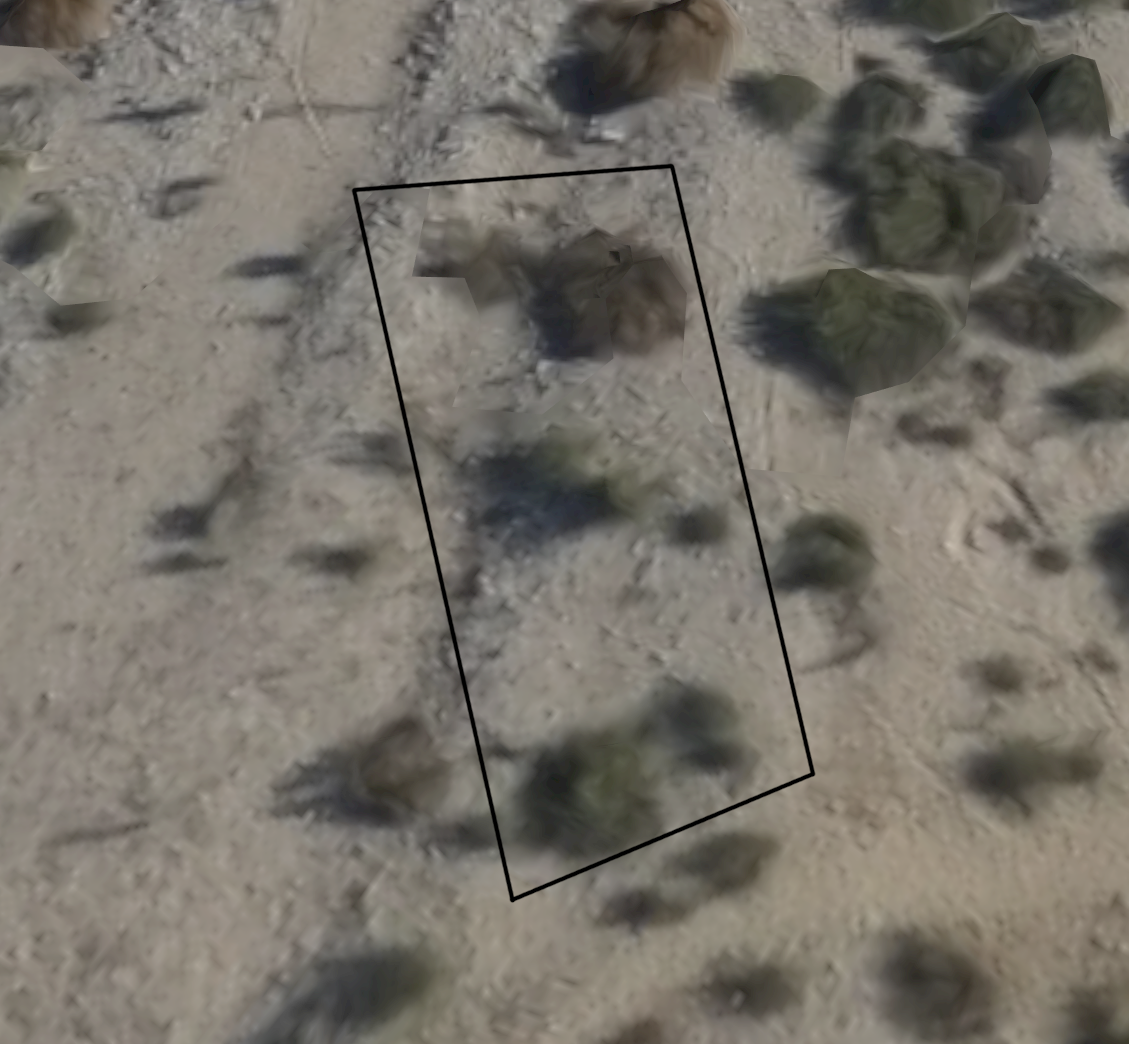
\includegraphics[scale=0.2, angle=-12]{images/preparation/reference_map2.5m_annotated.png}
    \caption{Considered terrain patch in Gazebo simulation}
    \label{stereo_reference}
\end{figure}

\begin{figure}[ht!]
    \centering
    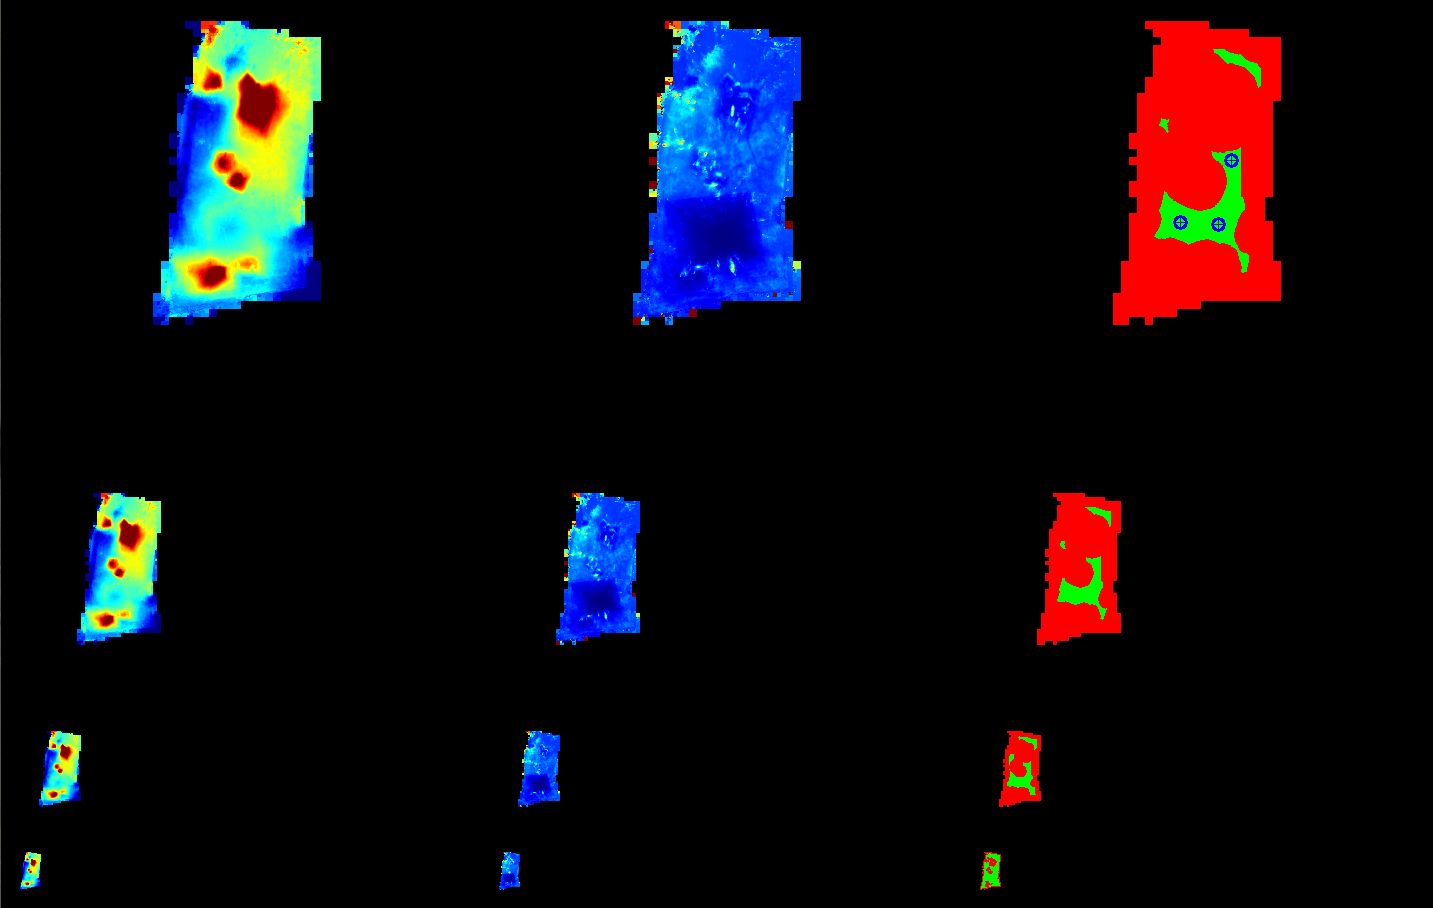
\includegraphics[scale=0.25]{images/preparation/stereo_2.5m.png}
    \caption{Stereo camera depth supplied LSD debug image at 2.5 m altitude}
    \label{qual_stereo_test}
\end{figure}

\clearpage %HERE

\begin{figure}[ht!]
    \centering
    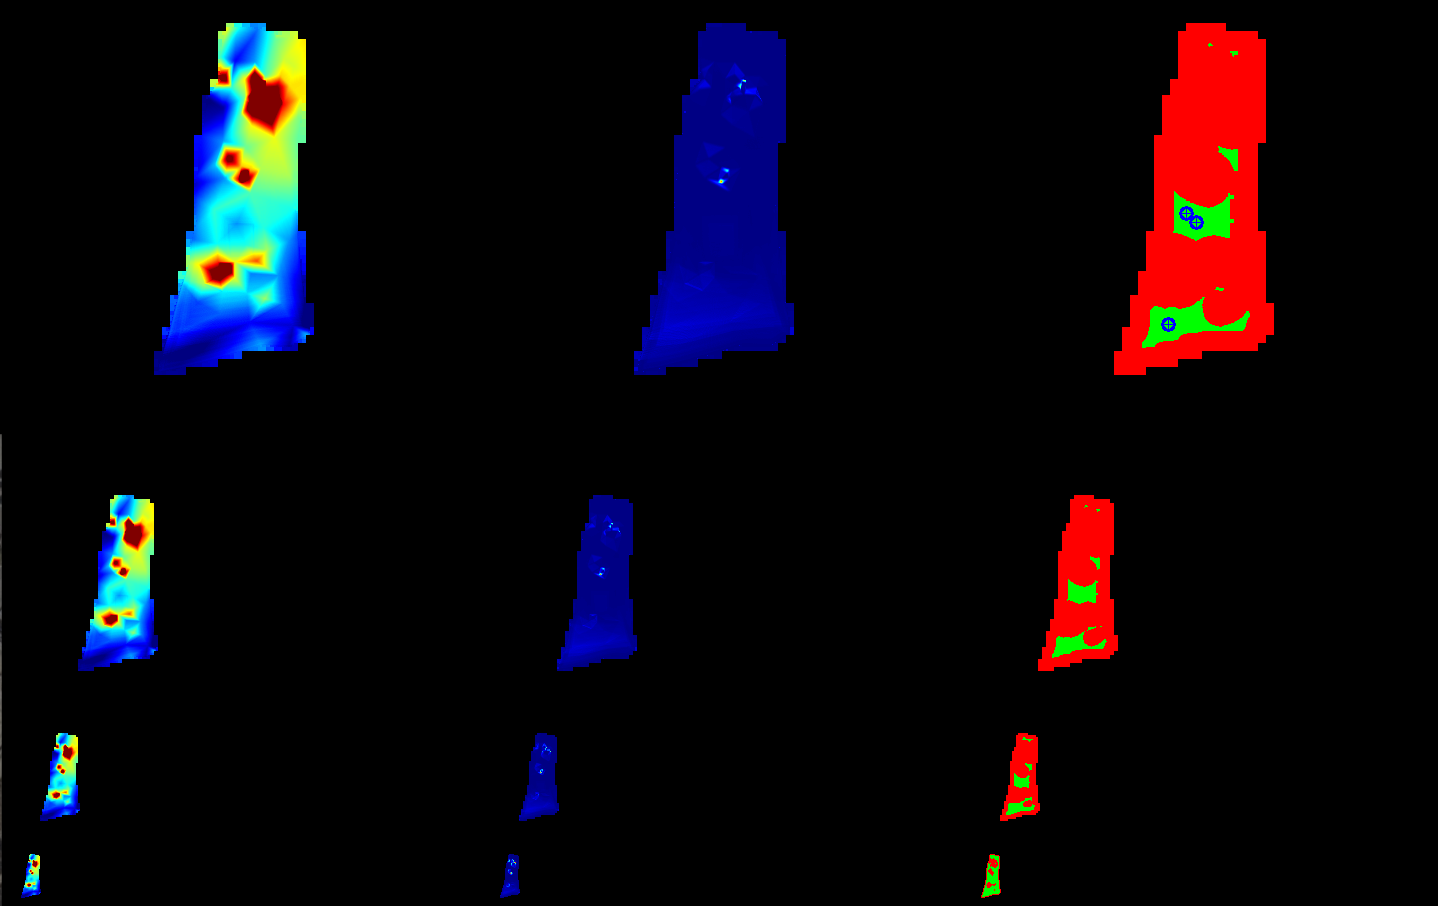
\includegraphics[scale=0.25]{images/preparation/GT_2.5m.png}
    \caption{GT depth supplied LSD debug image at 2.5 m altitude}
    \label{stereo_GT}
\end{figure}

When comparing the result to the ground truth LSD output it can be seen that LSD creates a very accurate DEM from the stereo camera depth input. The landing sites detected are reasonable when compared to the terrain reference. 

As the stereo camera has a relatively small, fixed baseline. The usage domain is restricted to low altitudes. The residual part of a mission is still flown using SFM. 

\subsubsection{StereoSGBM vs StereoBM}

To conclude the decision of the stereo method applied, hereafter are the two outputs of the StereoSGBM and StereoBM algorithms from OpenCV:

% TODO: Image of SteroSGBM vs StereoBM


